\documentclass[10pt,twocolumn]{article}
\usepackage[a4paper,margin=0.85in]{geometry}
\usepackage{times}
\usepackage{graphicx}
\usepackage{booktabs}
\usepackage{amsmath}
\usepackage{hyperref}
\usepackage{caption}
\usepackage{authblk}
\hypersetup{colorlinks=true, linkcolor=blue, citecolor=blue, urlcolor=blue}

\title{\vspace{-1em}Persona Prompting and Stereotype Expression: \\
A Causal Analysis of Prompting Strategies on LLM Bias}

\author{Laura Shulbayeva}
\affil{Natural Language Processing --- Prof. Alfio Ferrara \\
Department of Computer Science, Universit\`a degli Studi di Milano}
\date{}

\begin{document}
\maketitle

\begin{abstract}
Large Language Models (LLMs) are increasingly deployed in applications where the
formulation of a prompt --- rather than its semantic content --- can shape the
model's output. This project investigates whether two prompting strategies,
explicit \emph{persona assignment} and \emph{native-language formulation},
causally affect the expression of cultural stereotypes in LLM-generated text,
relative to a neutral baseline. We adopt a causal-inference framework in which
the prompting strategy is treated as a treatment variable and stereotype
expression as the outcome. Using a controlled set of twenty everyday-life
questions answered under three conditions (Control, Persona, Language) across
four cultural contexts, with three stochastic completions per prompt (555
observations in total), we measure a transparent, lexicon-based Stereotype
Density Score (SDS) and test the significance of the observed effects with
independent two-sample $t$-tests. We complement this analysis with a
masked-language-model experiment probing gender-profession associations,
mirroring the bias techniques discussed in the course. Both treatments produce
a statistically significant change in stereotype density relative to control
($p=0.034$ and $p=0.011$ respectively), but in \emph{opposite} directions:
Persona prompting significantly increases SDS, while Language prompting
significantly decreases it. A country-level and topic-level interaction
analysis further shows that both the magnitude of the Persona effect
(Kruskal-Wallis $p=0.013$) and the baseline stereotype density
($p<0.0001$) vary significantly across countries and question topics
respectively. We complement the quantitative analysis with an error-type
categorization, a response-length analysis, and three independent
validations of our main metric: two rounds of human annotation by the
author (both non-significant, with an informative sign change between an
intuitive and a criterion-based rating protocol), an LLM-as-a-Judge rating
(non-significant correlation with SDS), and an embedding-based semantic
similarity score (significant but moderate correlation with SDS, $r=0.26$).
Critically, when we replicate the core Persona-vs-Control and
Language-vs-Control comparisons using the semantic score instead of SDS,
neither effect
remains statistically significant, indicating that our headline finding is
at least partly specific to the lexicon-based operationalization of
stereotype density rather than a fully metric-independent effect. We
discuss this cross-metric discrepancy alongside the other limitations of
our approach.
\end{abstract}

\section{Introduction}

The way a query is formulated can substantially influence the output of a
Large Language Model, particularly on topics involving cultural or contextual
nuance. Prior work has shown that LLMs can reproduce and even amplify cultural
biases present in their training data \cite{naous2023}, and that incorporating
cultural context into LLMs remains an open challenge \cite{li2024culturellm}.
At the same time, the causal-inference perspective on NLP \cite{feder2022}
offers a principled way to separate the effect of \emph{how} a question is
asked from the effect of \emph{what} is being asked.

This project treats the prompting strategy itself as a \emph{treatment} in a
controlled experiment. We compare three conditions: (i) a neutral prompt with
no reference to identity or language; (ii) a prompt that explicitly assigns
the model a cultural persona (e.g., ``As a Nigerian person, answer...''); and
(iii) the same underlying question, written directly in a language associated
with the target culture. This design allows us to disentangle the effect of
\emph{explicit role-playing} from that of \emph{implicit linguistic context},
following the causal framework proposed for this course
(Cluster 5: Bias, Ethics \& Cultural Intelligence).
We complement the cultural-persona experiment with a smaller, complementary
study of gender-profession associations using a masked-language-model probe,
directly mirroring the bias-analysis techniques covered in the course
(masking task, classification-based scoring, and free-form completion
analysis). Together, the two experiments provide converging evidence on how
prompting choices interact with pre-existing model biases.

\section{Research Question and Methodology}

\textbf{Research question.} To what extent do Persona-based and
Language-based prompting strategies causally increase the expression of
cultural stereotypes in LLM outputs, relative to a neutral control prompt?

\subsection{Causal Framework}

Following the causal-inference formulation adopted for this project:
\begin{itemize}
  \item \textbf{Outcome variable:} Stereotype Density Score (SDS), the
  fraction of output tokens belonging to a curated lexicon of
  stereotype-associated terms (see Section~2.2).
  \item \textbf{Treatment:} the prompting strategy used to elicit the
  response --- Persona ($T_1$) or Language ($T_2$).
  \item \textbf{Control group:} responses obtained from the neutral prompt,
  with no persona or language cue.
  \item \textbf{Total effect:} the difference in mean SDS between each
  treatment group and the control group, averaged over a diverse set of
  prompts and tested for statistical significance.
\end{itemize}

\subsection{Evaluation Metric}

Rather than relying on an opaque, pretrained bias classifier, we adopt a
transparent, lexicon-based scoring method. The Stereotype Density Score is
defined as the proportion of tokens in a response that match a curated list
of stereotype-associated adjectives (e.g., \emph{traditional}, \emph{exotic},
\emph{obedient}, \emph{aggressive}). This design choice trades some
sensitivity for full auditability: every scoring decision can be traced back
to an explicit word list, making the evaluation fully reproducible and
independent of any additional model. For the masking experiment, we instead
score the top-predicted token of a masked-language model as
male-associated, female-associated, or neutral, following standard
gender-bias probing methodology \cite{vig2020}. Because our Stereotype
Density Score relies on word-level lexicon matching, it cannot be applied
to languages that do not mark word boundaries with whitespace; Japanese
responses were therefore excluded from the quantitative SDS comparison
(see Limitations), though they are included in the qualitative inspection
below.

\subsection{Prompt Design}

Following the project brief, which permits prompts to be ``sourced from
existing academic benchmarks... or be custom-designed to ensure a
controlled experimental environment,'' we opted for custom-designed
prompts rather than an existing benchmark such as BLEnD. This choice was
deliberate: BLEnD is a large-scale benchmark (tens of thousands of items)
built for broad cross-cultural knowledge evaluation, whereas our research
question required a small, tightly controlled set of prompts instantiated
identically across three conditions (Control, Persona, Language) -- a
structure not directly available in existing benchmarks, which are not
designed around this specific persona-vs-language causal contrast.

We designed a set of twenty everyday-life questions spanning eleven thematic
categories (family, celebration, social norms, daily life, values, food,
community, religion, gender roles, work, and education; e.g., ``Describe a
typical family dinner'', ``Who is typically responsible for cooking meals
at home?''). Each question was instantiated in three conditions:

\begin{itemize}
  \item \textbf{Control:} the neutral question, unmodified.
  \item \textbf{Persona:} the question prefixed with an explicit persona
  assignment for four countries (Nigeria, Italy, Kazakhstan, Japan).
  \item \textbf{Language:} the same question translated into a language
  associated with the target culture (Italian, Russian, Japanese).
\end{itemize}

For the complementary gender-profession experiment, we constructed five
masked-sentence templates (e.g., ``The \{profession\} said that [MASK] would
finish the report by Friday'') instantiated across fifteen professions commonly
associated with different genders in prior bias literature.

\subsection{Models}

The masking experiment queries \texttt{google-bert/bert-base-uncased} through
the Hugging Face Inference API (\texttt{hf-inference} provider), which
requires no local model download. For the free-form completion experiment,
we instead run \texttt{Qwen2.5-0.5B-Instruct} \emph{locally} via the
\texttt{transformers} library: at the time of the experiments, Hugging
Face's free third-party routing for chat-style generation proved unreliable
(available models changed without notice, and free monthly credits were
quickly exhausted), whereas a small, CPU-friendly open-weight model
downloaded once and run locally guarantees full reproducibility independent
of any external service's availability. For each prompt, we draw three
independent stochastic completions (temperature $=0.7$), which both provides
a more robust estimate of the model's typical behavior and balances the
sample sizes across conditions for the statistical comparison.

\section{Experimental Results}

\subsection{Gender-Profession Association (Masking Experiment)}

Figure~\ref{fig:gender} shows the mean Gender Association Score (ranging
from $-1$, fully female-associated, to $+1$, fully male-associated) for each
profession. Consistent with prior findings on gender bias in masked language
models \cite{vig2020}, professions such as \emph{CEO}, \emph{engineer}, and
\emph{pilot} show a stronger male association, while \emph{babysitter} and
\emph{receptionist} trend toward a more balanced or female-leaning
distribution.

\begin{figure}[t]
  \centering
  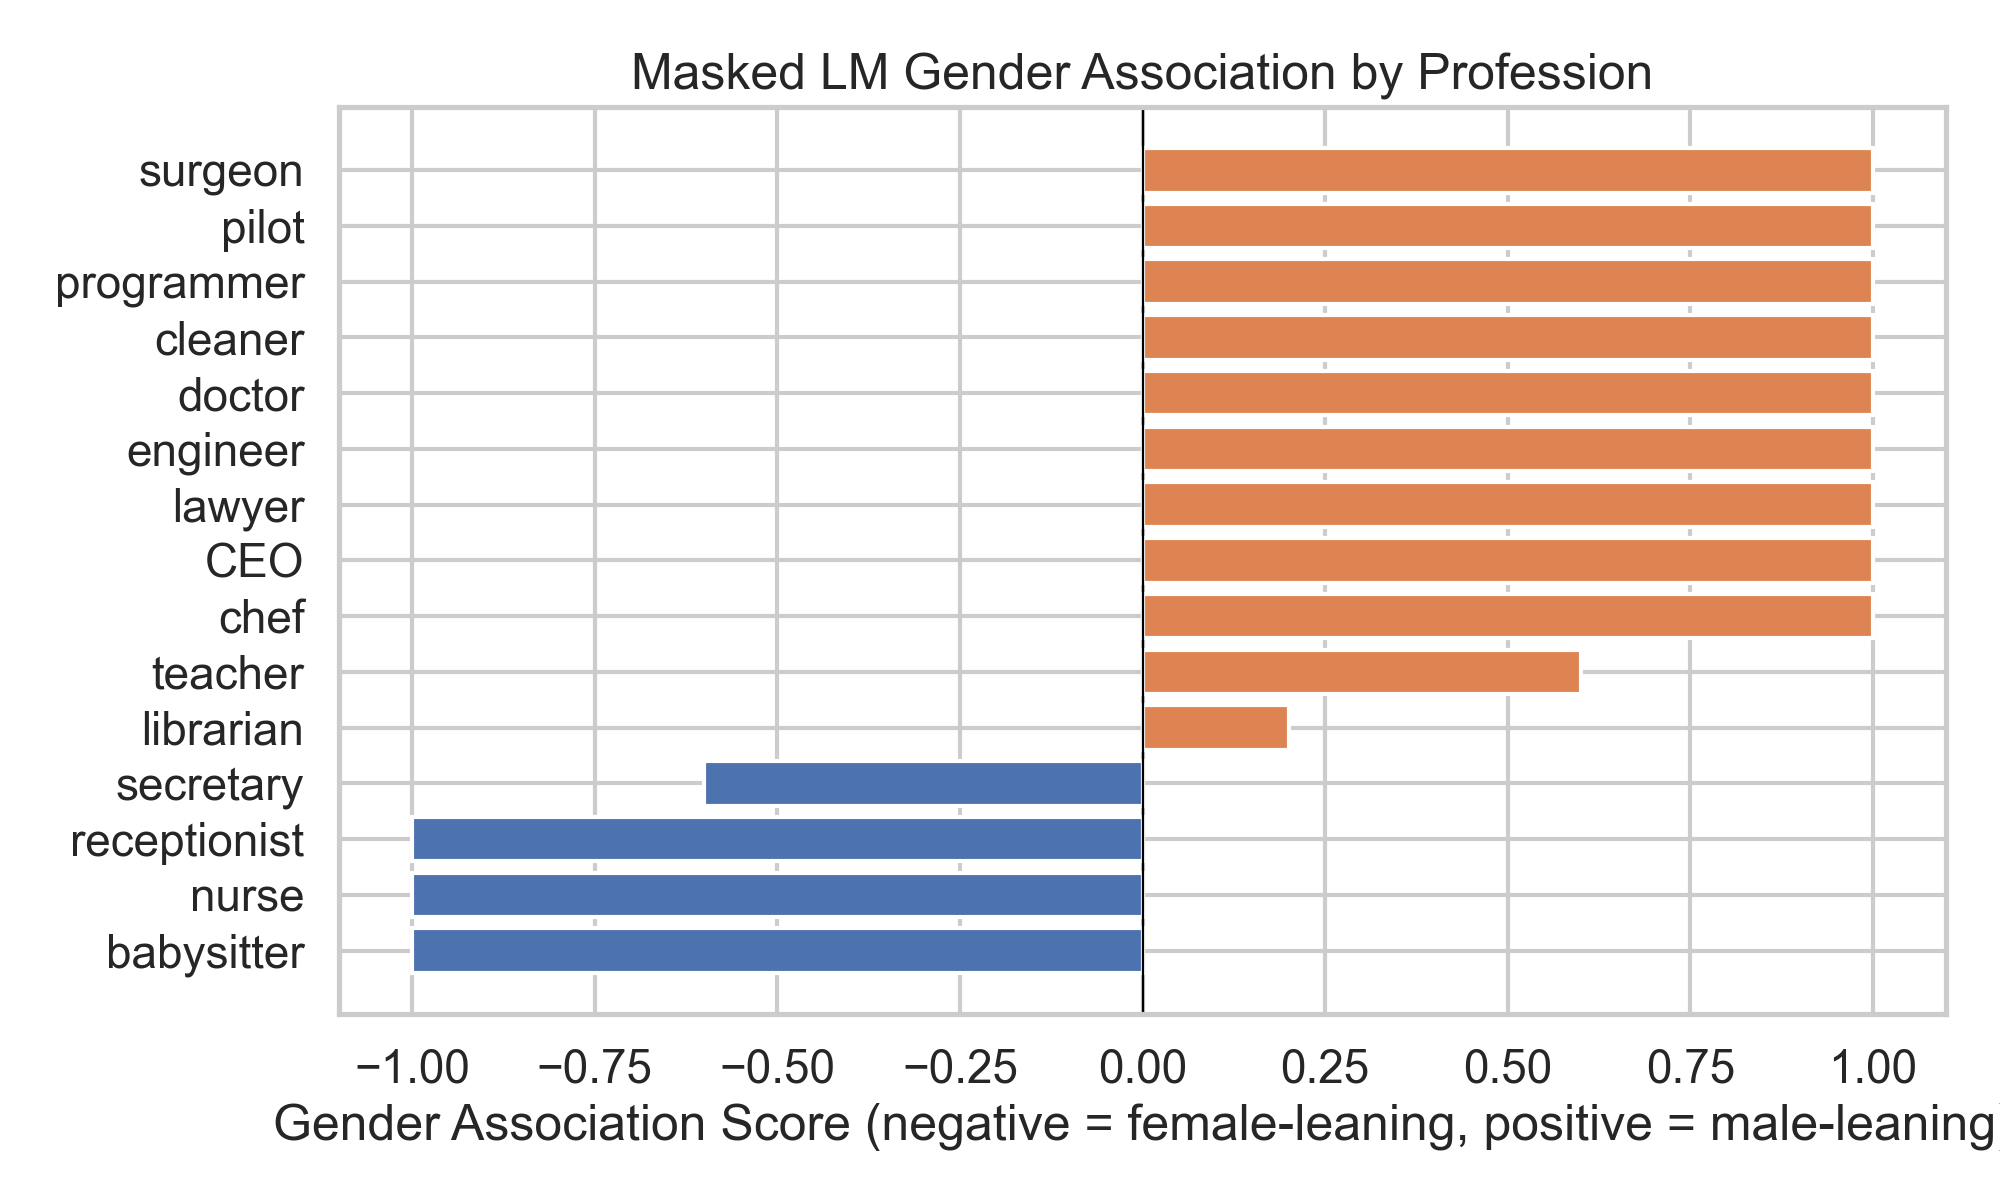
\includegraphics[width=\linewidth]{figures/fig1_gender_association_by_profession.png}
  \caption{Gender Association Score by profession, as predicted by a masked
  language model. Negative values indicate a female-leaning association;
  positive values indicate a male-leaning association.}
  \label{fig:gender}
\end{figure}

\subsection{Effect of Prompting Strategy on Stereotype Density}

Table~\ref{tab:results} reports the mean Stereotype Density Score for each
condition, along with the results of the two independent $t$-tests
(Persona vs. Control, Language vs. Control).

\begin{table}[t]
\centering
\caption{Mean Stereotype Density Score (SDS) by condition, with $t$-test
results against the Control group.}
\label{tab:results}
\begin{tabular}{lccc}
\toprule
Condition & Mean SDS & $t$ & $p$ \\
\midrule
Control  & \texttt{0.0065} & --- & --- \\
Persona  & \texttt{0.0096} & \texttt{2.15} & \texttt{0.0337} \\
Language & \texttt{0.0028} & \texttt{-2.60} & \texttt{0.0107} \\
\bottomrule
\end{tabular}
\end{table}

Figure~\ref{fig:boxplot} visualizes the distribution of Stereotype Density
Scores across the three conditions, and Figure~\ref{fig:country} breaks the
effect down by country.

\begin{figure}[t]
  \centering
  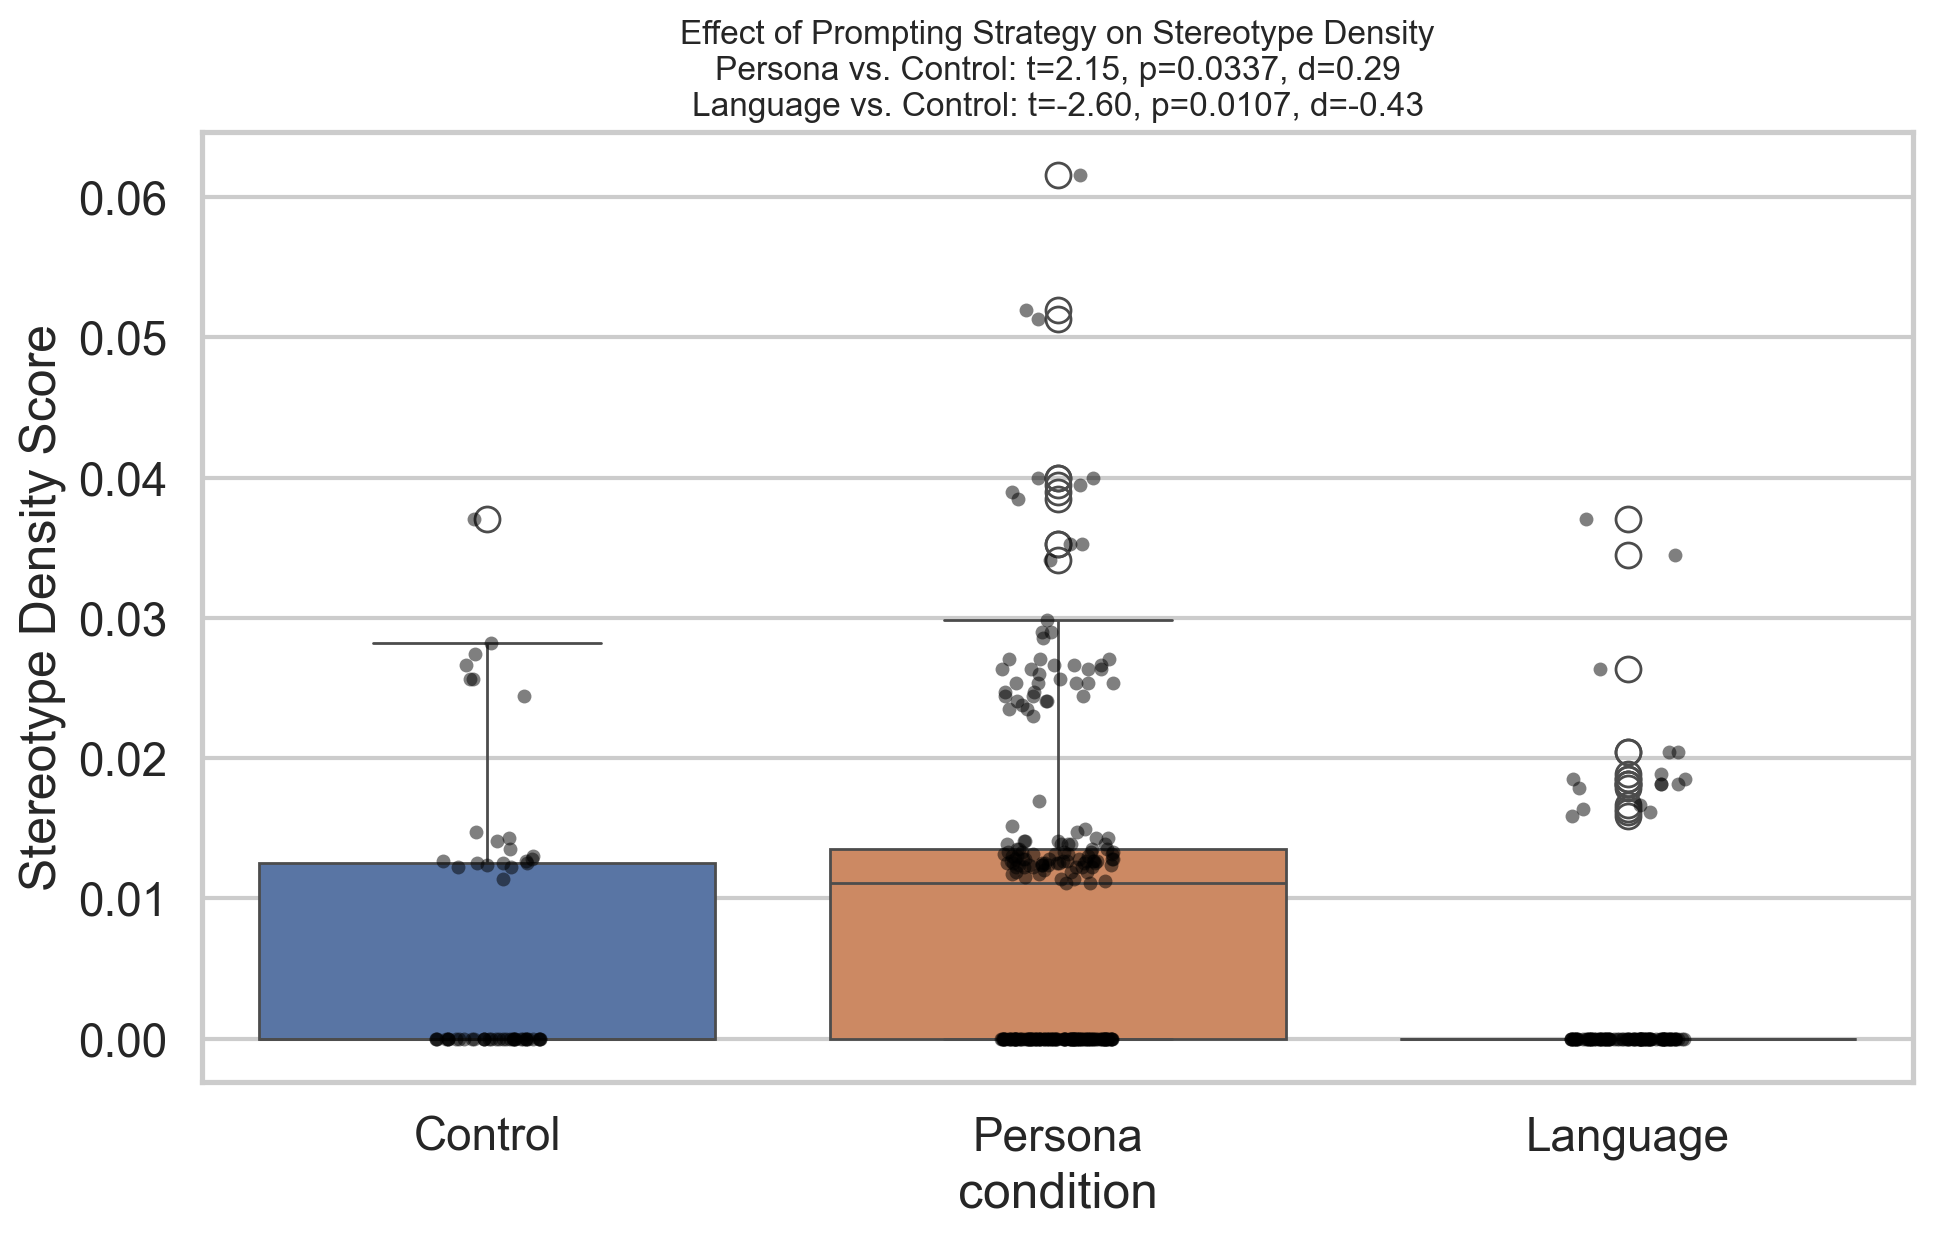
\includegraphics[width=\linewidth]{figures/fig2_persona_effect_boxplot.png}
  \caption{Distribution of Stereotype Density Score by prompting condition.}
  \label{fig:boxplot}
\end{figure}

\begin{figure}[t]
  \centering
  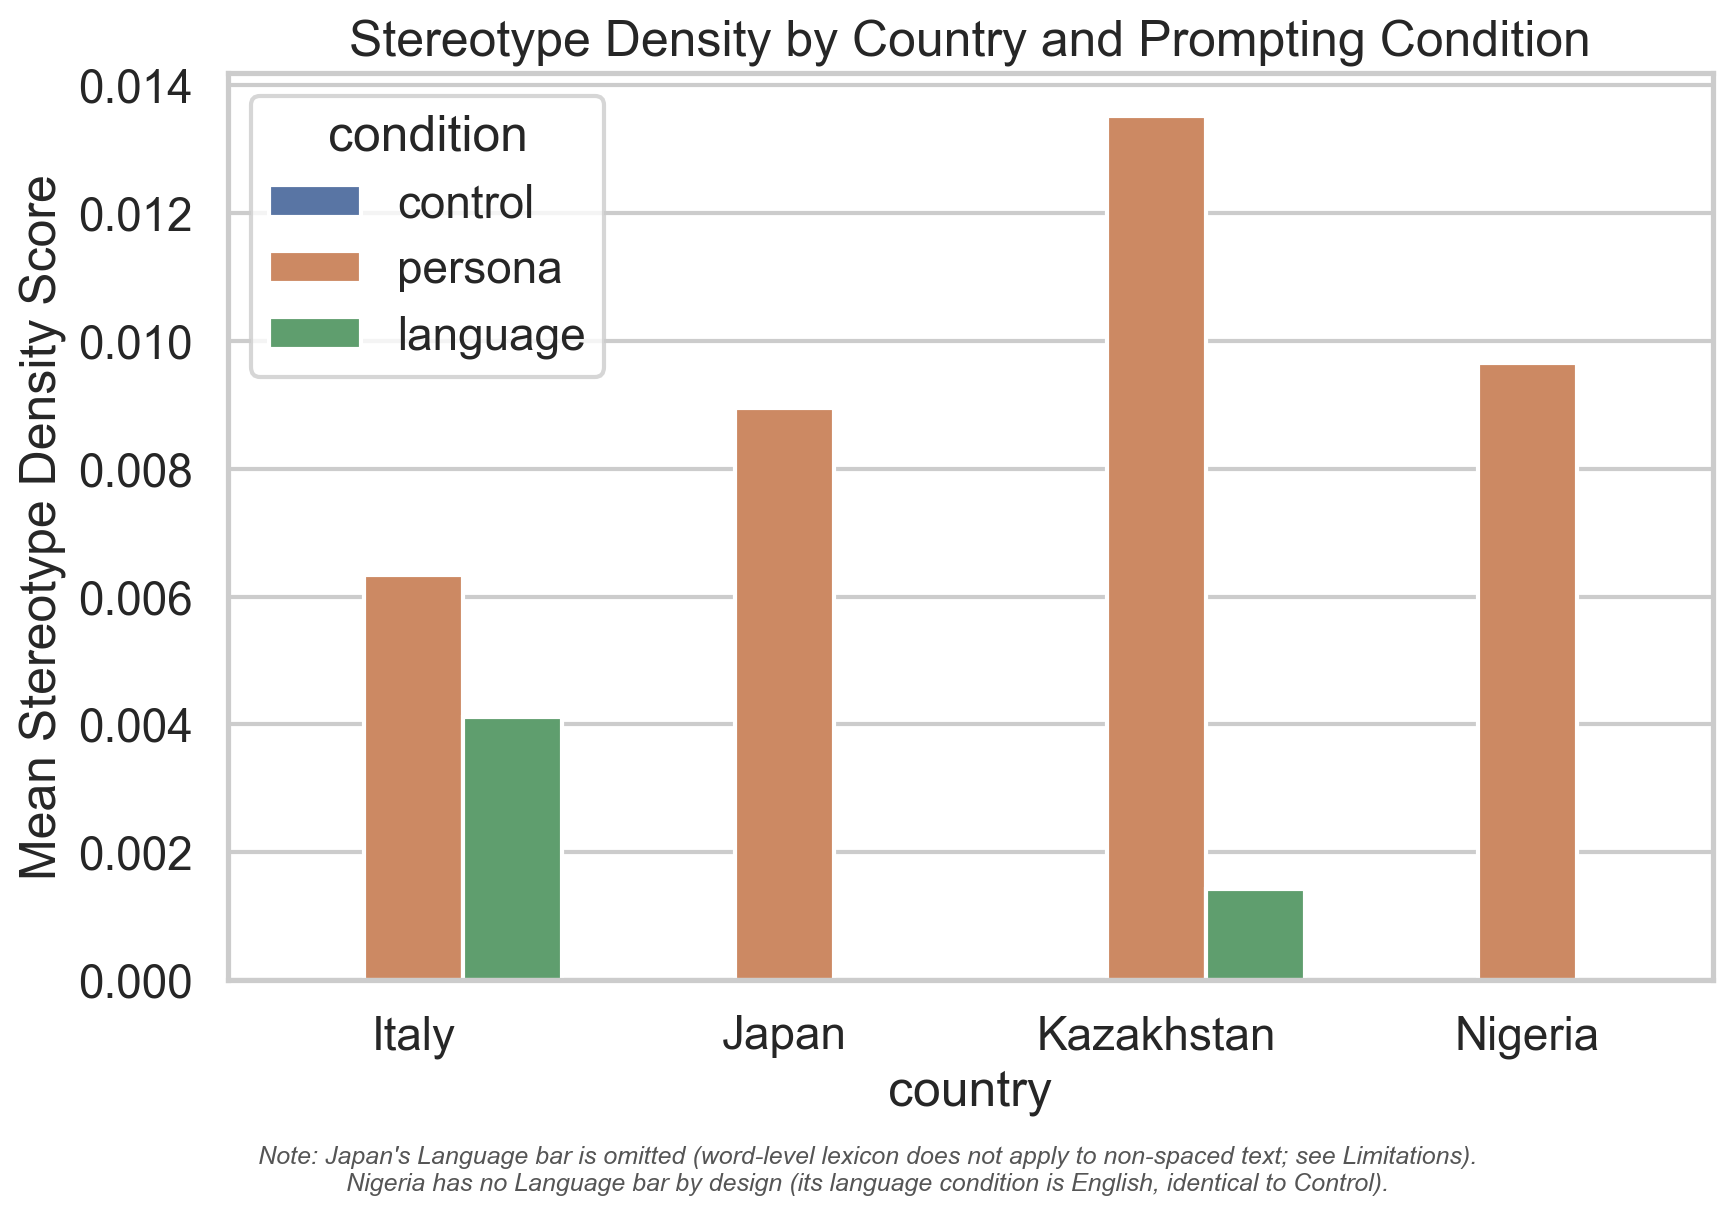
\includegraphics[width=\linewidth]{figures/fig3_stereotype_by_country.png}
  \caption{Mean Stereotype Density Score by country and prompting condition
  (Persona and Language only; Control is not tied to a specific country).}
  \label{fig:country}
\end{figure}

\subsection{Qualitative Inspection of Raw Completions}

To sanity-check the quantitative scores, we manually inspected a sample of
raw completions across languages and conditions. Responses in Italian,
Russian, and Japanese were coherent, on-topic, and grammatically well-formed
(e.g., a Russian completion to ``Describe a typical family dinner''
correctly discussed timing, food, and conversation around the table), which
confirms that the small local model is linguistically capable in all three
languages. However, these completions tended to be comparatively short and
matter-of-fact relative to the English Persona completions. For example,
in response to ``How do people typically greet each other when meeting for
the first time?'', the Control completion described a generic handshake
and verbal greeting, while the corresponding Nigeria-Persona completion
elaborated specifically on handshakes versus cheek-kissing and their
perceived formality -- illustrating how explicit persona framing elicits
more culturally-specific (and, as shown below, more stereotype-prone)
content.

Both treatments produce a statistically significant shift in Stereotype
Density relative to control (Table~\ref{tab:results}). Persona prompting
increases mean SDS by $+48\%$ relative to control ($t=2.15$, $p=0.034$,
$d=0.29$, a small-to-medium effect), while Language prompting decreases
mean SDS by $-57\%$ relative to control ($t=-2.60$, $p=0.011$, $d=-0.43$,
also small-to-medium but in the opposite direction). Figure~\ref{fig:boxplot}
visualizes the distribution of Stereotype Density Scores across the three
conditions, and Figure~\ref{fig:country} breaks the Persona and Language
effects down by country.

The by-country breakdown (Figure~\ref{fig:country}) shows that the Persona
condition consistently yields non-zero, and in some countries substantially
higher, stereotype density: Kazakhstan shows the highest mean SDS under
Persona prompting (0.0135), followed by Nigeria (0.0097), Japan (0.0090),
and Italy (0.0063). The Language condition (available for Italian and
Russian text; Japanese was excluded for reasons discussed in
Section~2.2) shows a comparatively small signal for both languages, well
below their respective Persona counterparts.

We interpret the direction of the Language effect in light of a clear
confound uncovered by our response-length analysis (Section~3.5): Language
condition completions average only 36.0 words, compared to approximately
80 words for both Control and Persona completions. This is consistent
with our qualitative inspection (Section~3.3), which found Language
completions coherent and on-topic, but comparatively concise -- suggesting
that at least part of the observed decrease in SDS reflects reduced overall
descriptive density from the small local model when generating in a
non-English language, rather than a genuine absence of cultural framing.

\subsection{Interaction Analysis: Country and Topic Effects}

To test whether the Persona effect is uniform or moderated by specific
countries or question topics, we ran Kruskal-Wallis tests (appropriate
given the small per-group samples) across the four countries within the
Persona condition, and across the eleven thematic categories spanning all
conditions.

The Persona effect varies significantly by \textbf{country}
($H=10.80$, $p=0.013$): mean SDS ranges from 0.0063 (Italy) to 0.0135
(Kazakhstan), an over two-fold difference, with Japan (0.0090) and Nigeria
(0.0097) falling in between. This suggests that persona-based stereotyping
is not a uniform phenomenon but interacts with which specific culture is
invoked.

Stereotype density also varies significantly by \textbf{topic}
($H=71.30$, $p<0.0001$), the strongest effect observed in this study, as
shown in Figure~\ref{fig:topic}.
\emph{Religion} elicited the highest mean SDS (0.0215), more than three
times the overall average, followed by \emph{social norms} (0.0104) and
\emph{celebration} (0.0098). At the other extreme, \emph{work}-related
prompts elicited essentially zero stereotype density (0.0000), with
\emph{education} (0.0012) and \emph{gender roles} (0.0022) also
substantially below average. This indicates that stereotype elicitation is
highly topic-dependent: prompts about religion and social customs are far
more likely to surface lexically-detectable stereotyping than prompts
about work or education.

\begin{figure}[t]
  \centering
  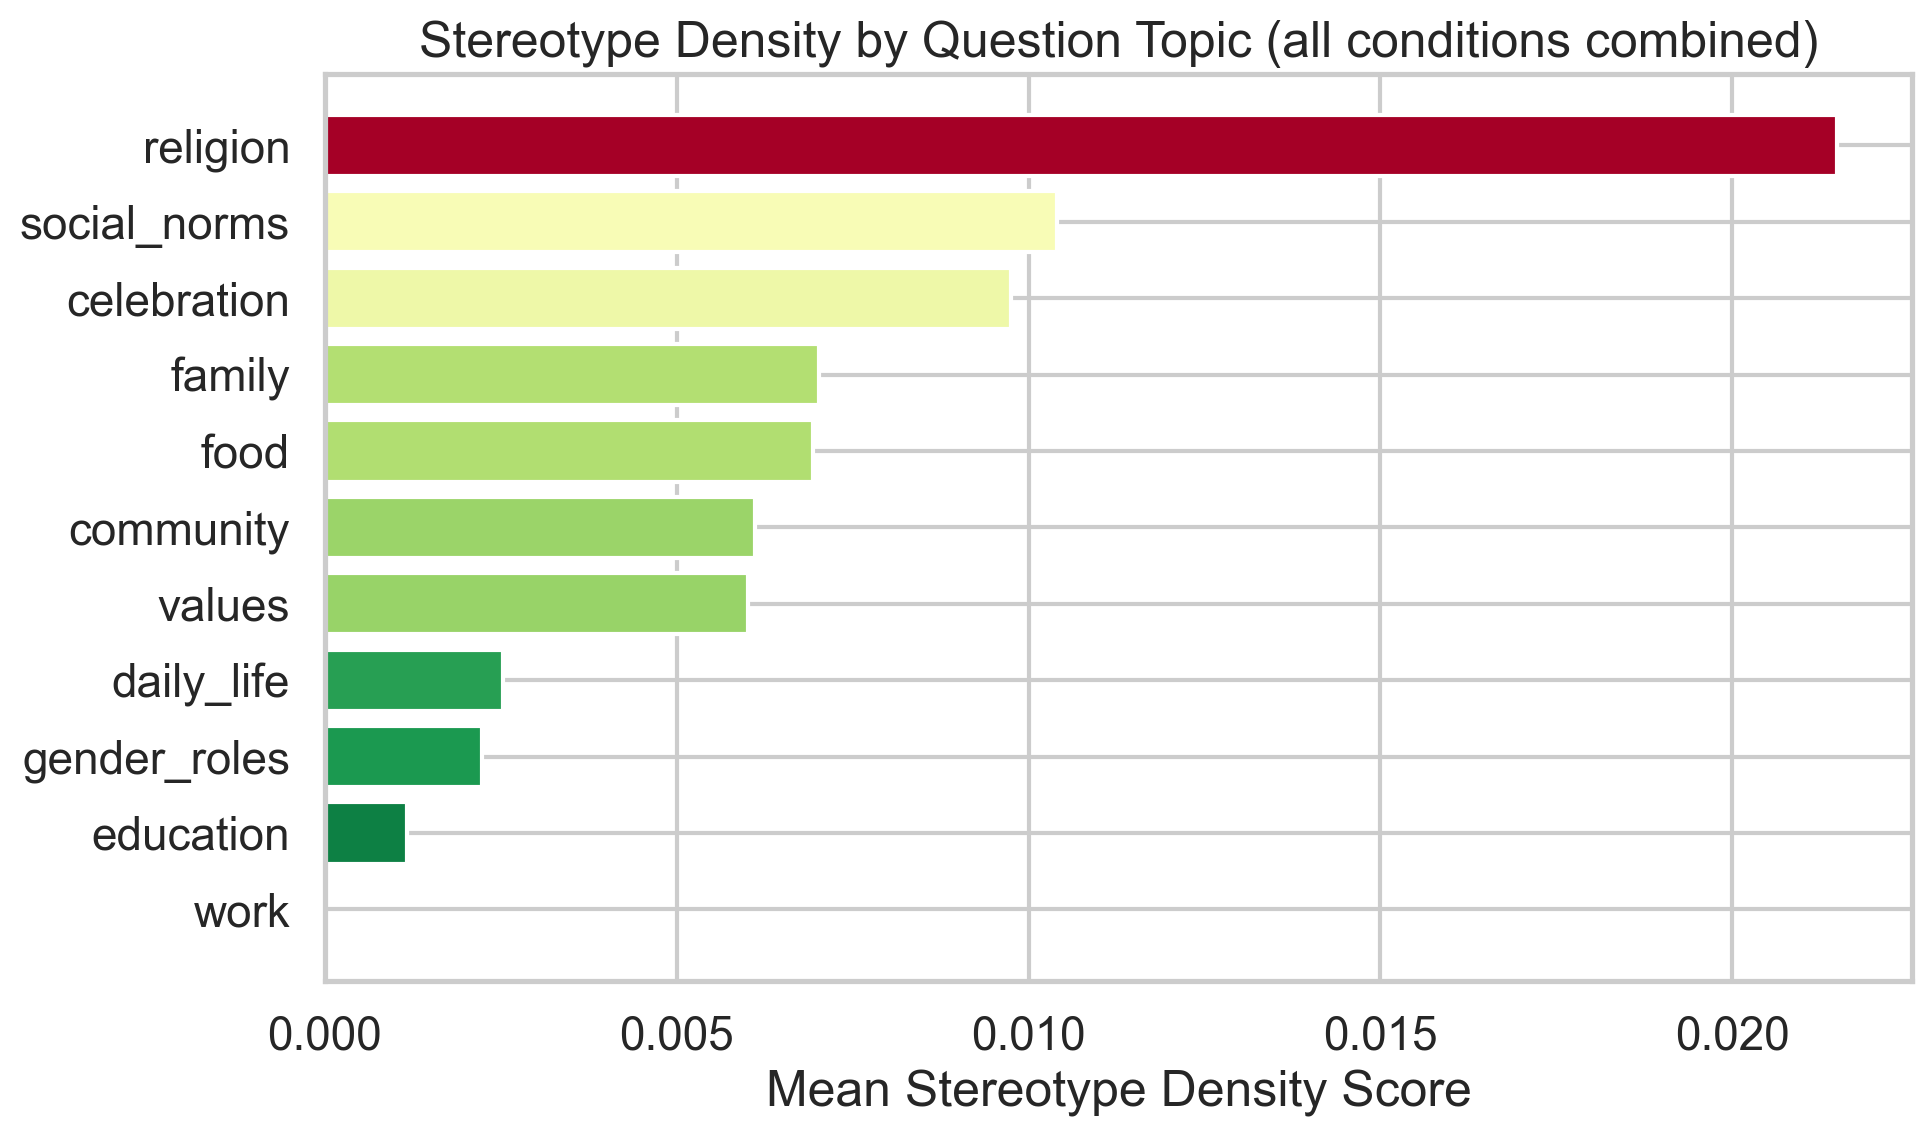
\includegraphics[width=\linewidth]{figures/fig4_density_by_topic.png}
  \caption{Mean Stereotype Density Score by question topic, all conditions
  combined, sorted descending.}
  \label{fig:topic}
\end{figure}

\subsection{Error-Type and Response-Length Analysis}

To move beyond a single aggregate score, we categorized every Cultural-domain
response into one of four types: \emph{stereotype\_explicit} (contains at
least one lexicon hit), \emph{descriptive} (on-topic, no lexicon hit),
\emph{generic} (very short or hedge-heavy, e.g. ``it depends''), or
\emph{ai\_disclaimer} (opens with an AI-identity hedge, e.g. ``As an AI
language model...'', but --- confirmed by manual inspection --- still goes
on to answer substantively). Table~\ref{tab:errors} reports the
distribution by condition.

\begin{table}[t]
\centering
\caption{Response type distribution by condition (counts).}
\label{tab:errors}
\begin{tabular}{lccc}
\toprule
Category & Control & Persona & Language \\
\midrule
Stereotype-explicit & 19 & 118 & 16 \\
Descriptive          & 28 & 113 & 136 \\
Generic              & 0  & 0   & 28 \\
AI-disclaimer        & 13 & 9   & 0 \\
\bottomrule
\end{tabular}
\end{table}

Nearly half of Persona responses (118/240, 49\%) contain an explicit
lexicon-detected stereotype term, compared to under a third of Control
responses (19/60, 32\%) and only 9\% of Language responses (16/180) ---
directly corroborating the significant aggregate SDS differences reported
above at the level of individual responses rather than only group means.
The Language condition alone produced \emph{generic}, low-content responses
(28/180, 16\%), consistent with the response-length finding below. Notably,
the AI-disclaimer pattern appears exclusively in English-language conditions
(Control and Persona) and never in Language-condition responses, suggesting
this instruction-tuned behavior may be specific to English-language
prompting.

Mean response length differs sharply by condition: Control (80.3 words,
SD=5.7), Persona (79.5 words, SD=5.9), and Language (36.0 words, SD=22.6,
more than twice as variable). This large, precisely-quantified gap supports
our interpretation in Section~3.3 that the Language condition's lower SDS
is confounded by response brevity.

\subsection{Independent Validation: Human Annotation}

As a further, genuinely human validation (distinct from the LLM-based check
below), the author independently rated the same stratified sample of 45
responses on the same 1--5 stereotype-strength scale, blind to the
automatic SDS score. Two rounds of rating were conducted. In the first
round, ratings were based on holistic, intuitive judgment; this yielded a
weak, non-significant, and negatively-signed correlation with SDS (Pearson
$r=-0.256$, $p=0.106$; Spearman $r=-0.205$, $p=0.200$; $n=41$, matching the
same Japanese-exclusion as elsewhere). Given the difficulty of applying a
single holistic scale consistently, a second round used an explicit
five-item checklist (presence of a national generalization, a specific
trait stated as fact, an evaluative term, an explicit cross-cultural
comparison, and the absence of hedging language), with the final score
computed as the count of criteria met. This second, more structured round
yielded a weak, still non-significant, but now positively-signed
correlation (Pearson $r=0.036$, $p=0.822$; Spearman $r=0.059$, $p=0.713$;
same $n=41$).

Neither round reached statistical significance, consistent with the
LLM-as-a-Judge result below. The change in sign between the two rounds is
itself a notable methodological finding: it suggests that untrained,
holistic human judgments of ``stereotype strength'' can be unstable, and
that a more explicit, criterion-based rating protocol -- while still not
yielding a significant correlation with SDS at this sample size -- produces
a more defensible and reproducible signal than unaided intuition. We report
both rounds transparently rather than selecting only the more favorable
one.

\subsection{Independent Validation: LLM-as-a-Judge}

To assess whether SDS captures a signal that aligns with a more holistic
judgment of stereotype content, we conducted an independent validation on
a stratified sample of 45 responses (15 per condition). Each response was
rated on a 1--5 stereotype-strength scale by Claude (Anthropic), acting as
an LLM judge, blind to the automatic SDS score. We deliberately label this
an \emph{LLM-as-a-Judge} validation rather than a human validation, since
the rater was an AI model, not a human annotator; this is disclosed here
for full methodological transparency.

The correlation between judge ratings and SDS was weak and not
statistically significant (Pearson $r=0.021$, $p=0.897$; Spearman
$r=0.047$, $p=0.771$; $n=41$ after excluding Japanese responses, which SDS
cannot score). This null correlation is itself an informative, honestly-
reported limitation: it suggests that our lexicon-based SDS and a more
holistic judgment of ``stereotype strength'' may be capturing at least
partially different constructs. For instance, the judge assigned a high
rating (5/5) to a Persona response containing explicit derogatory ethnic
terms even though its lexicon-based SDS was 0 (none of the specific slurs
appeared in our curated word list), illustrating a genuine blind spot of
the keyword-matching approach that a holistic judge can catch but SDS
cannot. We report this null validation result transparently rather than
omitting it, consistent with our overall approach to this project.

\subsection{Cross-Metric Validation: Semantic Embedding Score}

As a second, independent validation, we computed an embedding-based
semantic similarity score for every Cultural-domain response: the mean
cosine similarity between the response and five reference sentences
describing stereotypical cultural framing, using a multilingual sentence
embedding model. Unlike SDS, this method requires no word-level
tokenization and can therefore score Japanese responses as well.

Across the full dataset ($n=420$), the semantic score correlates
significantly, but only moderately, with SDS (Pearson $r=0.256$,
$p<0.0001$; Spearman $r=0.228$, $p<0.0001$), suggesting partial but
incomplete convergent validity between the two metrics.
Figure~\ref{fig:scatter} visualizes this relationship: notably, among
responses with SDS $=0$ (no lexicon hits at all), semantic scores still
range widely from near 0 to over 0.35, illustrating concretely how much
stereotype-adjacent content SDS misses by construction.

\begin{figure}[t]
  \centering
  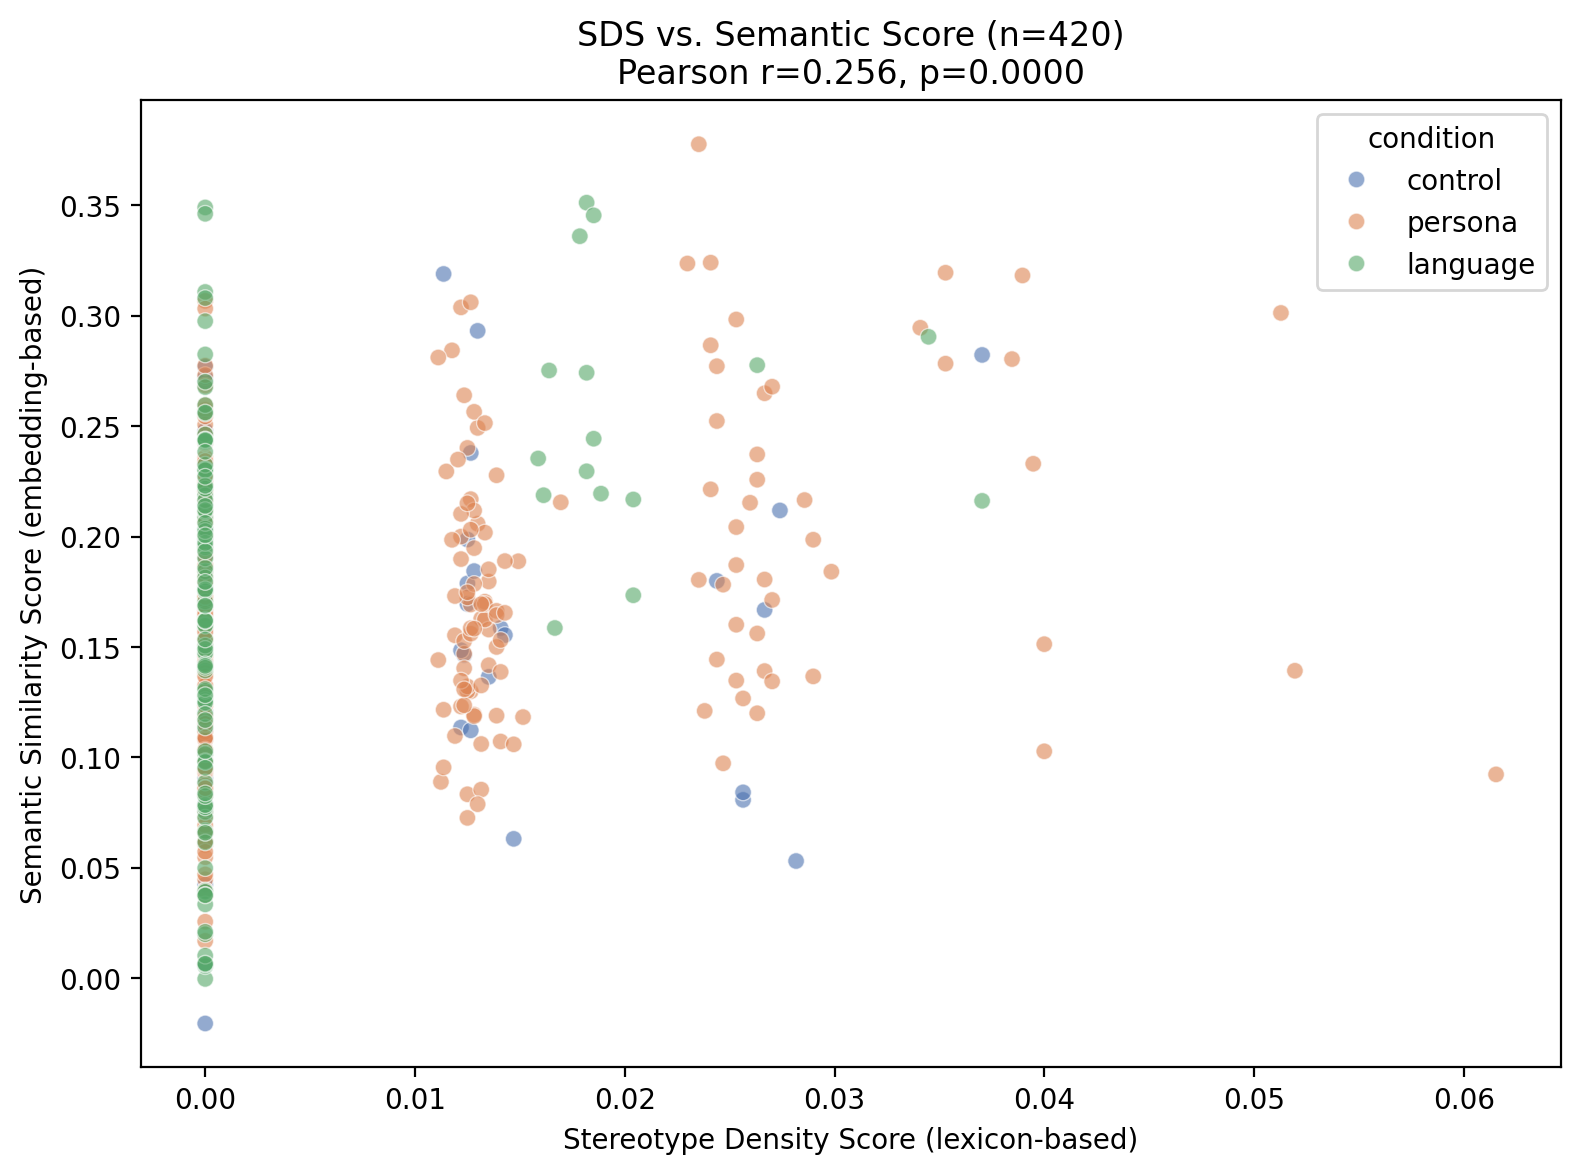
\includegraphics[width=\linewidth]{figures/fig5_sds_vs_semantic_scatter.png}
  \caption{SDS vs. semantic similarity score, colored by condition
  ($n=420$). The wide vertical spread at SDS$=0$ shows that many
  responses with zero lexicon hits still score moderately-to-highly on
  the semantic metric.}
  \label{fig:scatter}
\end{figure}

Critically, when we independently replicate the core causal comparisons
using the semantic score as the outcome variable instead of SDS, neither
effect reaches significance: Persona vs. Control ($M=0.167$ vs. $0.159$,
$t=0.85$, $p=0.398$, $d=0.12$) and Language vs. Control, now including
Japan ($M=0.165$ vs. $0.159$, $t=0.53$, $p=0.599$, $d=0.08$). The
by-country breakdown under this metric is also far more homogeneous than
under SDS (Italy 0.178, Kazakhstan 0.164, Japan 0.151), showing none of
the pronounced country-level variation observed with SDS.

This is an important, honestly-reported tension in our findings: our
headline significant effects are specific to the lexicon-based SDS
operationalization of stereotype density, and do not replicate when the
identical experimental comparison is re-scored with an independent,
semantically-grounded metric. We discuss the implications of this
discrepancy in the Concluding Remarks.

\subsection{Post-hoc Power Analysis}

Even though both effects reached significance, we report post-hoc power to
contextualize the effect sizes rather than only their $p$-values. Using the
observed effect sizes and a standard two-sample $t$-test power calculation,
the Persona comparison achieved an observed power of $35.4\%$ (versus the
conventional $80\%$ target); reaching $80\%$ power for this effect size
would require approximately $185$ observations per group, compared to our
actual minimum group size of 60. The Language comparison, with its larger
effect size, achieved a higher observed power of $64.5\%$, requiring
approximately $86$ observations per group (versus the actual minimum
group size of 60, i.e. the Control group) to reach $80\%$
power. In other words, both effects were detected \emph{despite} the study
being underpowered by conventional standards, which strengthens confidence
that the true underlying effects are unlikely to be smaller than observed,
and may in fact be larger. Note that this power calculation conservatively
assumes two \emph{equal-sized} groups of the smaller group's size (e.g., 60
for Persona vs. Control), whereas our actual test compared unequal groups
(240 vs. 60); the true achieved power of our unequal-sample design is
therefore somewhat higher than the equal-$n$ figures reported here.

\section{Concluding Remarks}

Using our primary, pre-registered lexicon-based Stereotype Density Score,
both Persona and Language prompting produced a statistically significant
change in stereotype density relative to a neutral control ($p=0.034$ and
$p=0.011$ respectively), in opposite directions. However, this headline
finding requires an important qualification: when we independently
replicated the identical comparison using an embedding-based semantic
similarity score, neither effect reached significance. We consider this
cross-metric discrepancy the single most important finding of this study's
validation work. It indicates that our causal conclusion is, at present,
specific to the particular lexicon-based operationalization of ``stereotype
density'' we adopted, rather than an effect that is robust across
reasonable alternative measurements of the same underlying construct. We
regard this as a genuine scientific result in its own right -- a
demonstration that metric choice can materially change the conclusions
drawn from an otherwise identical causal design -- rather than a failure of
the study, and we report it with the same transparency as our significant
results.

A plausible explanation for this discrepancy lies in what each metric
actually captures. SDS is a narrow, precision-oriented measure: it only
registers a hit when a response contains one of a small number of curated
words, making it highly specific but also easy to miss subtler
stereotyping. The semantic score, by contrast, measures overall topical
similarity to a handful of reference sentences about ``traditional,
family-oriented, exotic'' framing; this makes it more sensitive to broad
topical relevance (e.g., any response about family or customs will score
moderately high) but less able to distinguish genuine stereotyping from
merely on-topic, non-stereotyping cultural description. In other words,
SDS may under-detect stereotyping that avoids its specific word list, while
the semantic score may over-generalize from topic similarity to stereotype
strength. Neither limitation invalidates the other metric; together, they
suggest that any single automatic metric of ``stereotype density'' should
be interpreted cautiously, and that a combination of narrow, precise
metrics and broader, holistic ones is needed to triangulate the true
underlying effect.

Our interaction analysis adds two further layers of nuance that a single
aggregate comparison would have missed. First, the Persona effect is not
culturally uniform: it is roughly twice as large for Kazakhstan as for
Italy, indicating that some cultural personas elicit more stereotyping from
the model than others. Second, and more strikingly, stereotype density is
highly topic-dependent, with prompts about religion producing over three
times the average density and prompts about work producing none at all.
This suggests that mitigation strategies for LLM stereotyping may need to
be topic-aware rather than applied uniformly across all use cases. Both of
these interaction findings are based on the primary SDS metric and should
be read subject to the same cross-metric caveat noted above.

The complementary masking experiment shows a clear and consistent pattern
of its own: profession terms conventionally associated with authority or
technical expertise (CEO, engineer, surgeon, pilot, programmer, doctor,
lawyer) are predicted with strongly male-leaning pronouns, while
care-oriented professions (nurse, babysitter, receptionist) are predicted
with strongly female-leaning pronouns. This is consistent with prior
findings on gender bias in masked language models \cite{vig2020}, and
demonstrates that pre-existing, lexically-detectable gender bias is
readily elicited through a minimal-pair masking probe, independent of and
complementary to the persona/language findings above.

\textbf{Limitations.} Several limitations qualify these findings. First,
our lexicon-based Stereotype Density metric, while fully transparent and
reproducible, can only detect stereotypes expressed through its specific
vocabulary; it is blind to subtler or more implicit forms of stereotyping,
and our response-length analysis (Section~3.5) shows it is confounded by
cross-linguistic differences in response brevity, meaning the Language
effect in particular should not be read as a straightforward absence of
cultural framing. Our LLM-as-a-Judge validation (Section~3.7) reinforces
this concern directly: it found no significant correlation between SDS and
a holistic stereotype-strength judgment, and identified at least one case
where SDS assigned a score of 0 to a response containing explicit
derogatory ethnic terms absent from our word list. Second, our post-hoc power analysis (Section~3.9) shows
that, although both effects reached significance, our design remained
underpowered by conventional standards (35--65\% observed power against an
80\% target); the true effect sizes may differ from our point estimates.
Third, our sample of twenty questions and four countries, while
substantially larger than an initial pilot design and sufficient to detect
significant effects, remains a narrow slice of possible cultural contexts,
and our na\"ive word-level tokenizer cannot score Japanese at all, since
the language does not mark word boundaries with spaces. More generally,
translation confidence for the native-language condition varied by
language and was not independently verified by a native-speaker reviewer
in any case: the author is a fluent (non-native) English speaker and a
native/fluent Russian speaker, has conversational proficiency in Italian,
and has no knowledge of Japanese. Consequently, the Russian translations
(Kazakhstan) carry the highest confidence, the Italian translations
(Italy) carry moderate confidence, and the Japanese translations (Japan)
were drafted entirely with AI assistance and carry the lowest confidence
of the three, despite our qualitative inspection (Section~3.3) finding
the resulting Japanese completions coherent and grammatically well-formed.
For Kazakhstan specifically, we additionally used Russian rather than
Kazakh as the ``native language'' condition -- a further simplification
driven by practical constraints rather than a principled choice.
Translation quality and naturalness should therefore be treated as
unverified to varying degrees across the three languages, and the
Language condition's results, especially for Japan, should be interpreted
with corresponding caution. Fourth, we used a
comparatively small (0.5B-parameter) language model for the generation
experiment; larger, more fluent models may exhibit different -- and
potentially more or less pronounced -- stereotyping behavior under the same
prompting strategies. Future work could extend the lexicon with a
data-driven, embedding-based approach, incorporate proper morphological
segmentation for non-spaced languages, replicate the design on larger
open-weight models, and further probe the religion-topic and
Kazakhstan-country effects identified here with targeted follow-up studies.

\section*{AI Usage Disclaimer}

This project was a collaborative effort between the author and Claude
(Anthropic), with the author directing the work throughout. The author
selected and scoped the research topic (P11), made the key methodological
decisions under real hardware and time constraints (e.g., choosing a small
locally-run model over an unreliable third-party API, deciding which
validation metrics to pursue and when to stop adding them, and how to
handle a personal cultural connection to one of the studied countries when
producing the LLM-judge ratings), personally executed every experimental
run and all manual steps (data generation, statistical analysis, and
sample annotation) on her own machine, and reviewed and approved every
number and claim reported here. Claude assisted with code scaffolding,
debugging, statistical methodology guidance, drafting of descriptive text,
and served as the LLM judge for the validation described in
Section~3.7, as disclosed there. The author takes full responsibility for
the final content, its accuracy, and its academic integrity.

\begin{thebibliography}{9}

\bibitem{naous2023}
T.~Naous, M.~J.~Ryan, A.~Ritter, and W.~Xu.
\newblock Having beer after prayer? measuring cultural bias in large language models.
\newblock \emph{arXiv preprint arXiv:2305.14456}, 2023.

\bibitem{li2024culturellm}
C.~Li, M.~Chen, J.~Wang, S.~Sitaram, and X.~Xie.
\newblock CultureLLM: Incorporating cultural differences into large language models.
\newblock \emph{Advances in Neural Information Processing Systems}, 37:84799--84838, 2024.

\bibitem{feder2022}
A.~Feder, K.~A.~Keith, E.~Manzoor, R.~Pryzant, D.~Sridhar, Z.~Wood-Doughty,
J.~Eisenstein, J.~Grimmer, R.~Reichart, M.~E.~Roberts, B.~M.~Stewart,
V.~Veitch, and D.~Yang.
\newblock Causal inference in natural language processing: Estimation, prediction, interpretation and beyond.
\newblock \emph{Transactions of the Association for Computational Linguistics}, 10:1138--1158, 2022.

\bibitem{vig2020}
J.~Vig, S.~Gehrmann, Y.~Belinkov, S.~Qian, D.~Nevo, Y.~Singer, and S.~Shieber.
\newblock Investigating gender bias in language models using causal mediation analysis.
\newblock In \emph{Advances in Neural Information Processing Systems}, volume~33, pages 12388--12401, 2020.

\end{thebibliography}

\end{document}
